% ^^A documentation part start with %
% ^^A All other parts are called definition parts
% ^^A Comments in documentation part
% ^^A equivalently use \iffalse ... \fi
% \iffalse meta-comment
% !TeX program = XeLaTeX
% !TeX encoding = UTF-8
%
% Copyright (C) 2016 by Van Abel <van141.abel(AT)gmail.com>
% ---------------------------------------------------------------------
%
% This work may be distributed and/or modified under the
% conditions of the LaTeX Project Public License, either
% version 1.3c of this license or (at your option) any later
% version. This version of this license is in
%    http://www.latex-project.org/lppl/lppl-1-3c.txt
% and the latest version of this license is in
%    http://www.latex-project.org/lppl.txt
% and version 1.3 or later is part of all distributions of
% LaTeX version 2005/12/01 or later.
%
% This work has the LPPL maintenance status `maintained'.
%
% The Current Maintainers of this work is Van Abel.
%
% ---------------------------------------------------------------------
%
%<*internal>
\iffalse
%</internal>
%<*readme>
---------------------------------------------------------------
mathexam --- A package for math exam
===============================================================
Released under the LaTeX Project Public License v1.3c or later
See http://www.latex-project.org/lppl.txt
---------------------------------------------------------------
This package is developed when I prepare the midterm exam in the Shanghai Jiao Tong University.
It based on the `multicol` package to create two column typesetting, and `eso-pic` package to 
add the basic infomation, such as the title, the score table, as a background image.

USAGE
---------------------------------------------------------------
Download the zip file and unzip to a local directory, then have a look at the
`mathexam-main.pdf`, you can edit and compile it by 
`latexmk -xelatex -shell-escape mathexam-main.tex`.
%</readme>
%<*internal>
\fi
\def\nameoflatex{plain}
\ifx\nameoflatex\fmtname\else
  \expandafter\begingroup
\fi
%</internal>
%
%<*install>

\input docstrip.tex
\keepsilent
\askforoverwritefalse
\preamble
----------------------------------------------------------------
mathexam --- 数学类考试出题宏包
===============================================================
E-mail: van141.abel(AT)gmail.com
Released under the LaTeX Project Public License v1.3c or later
See http://www.latex-project.org/lppl.txt
----------------------------------------------------------------

\endpreamble
\postamble

Copyright (C) 2009 by You <van141.abel(AT)gmail.com>

This work may be distributed and/or modified under the
conditions of the LaTeX Project Public License (LPPL), either
version 1.3c of this license or (at your option) any later
version.  The latest version of this license is in the file:

http://www.latex-project.org/lppl.txt

This work is "maintained" (as per LPPL maintenance status) by
You.

This work consists of the file  mathexam.dtx
and the derived files           mathexam.ins,
                                mathexam-main.tex,
                                mathexam-main.pdf,
                                mathexam-main-answer.tex,
                                mathexam-main-answer.pdf,
                                mathexam.pdf and
                                mathexam.sty.

\endpostamble
\generate{
  \usedir{tex/latex/mathexam}
  \file{\jobname.sty}{\from{\jobname.dtx}{package}}
  \nopreamble\nopostamble
  \file{main.tex}{\from{\jobname.dtx}{main}}
  \file{\jobname-main.tex}{\from{\jobname.dtx}{maintex}}
  \file{\jobname-main-answer.tex}{\from{\jobname.dtx}{mainanstex}}
  \usedir{doc/latex/mathexam}
  \file{README.txt}{\from{\jobname.dtx}{readme}}
}
\obeyspaces
\Msg{****************************************************}
\Msg{*                                                   }
\Msg{* To finish the installation you have to move the   }
\Msg{* following file into a directory searched by TeX   }
\Msg{* e.g. tex/latex/mathexam:                          }
\Msg{*                                                   }
\Msg{* \jobname.sty                                      }
\Msg{*                                                   }
\Msg{* To produce the documentation run the file         }
\Msg{* \jobname.dtx through XeLaTeX.                     }
\Msg{*                                                   }
\Msg{* To produce the sample file run the file           }
\Msg{* \jobname-main.tex or \jobname-main-answer.tex     }
\Msg{* through XeLaTeX and BibTeX                        }
\Msg{*                                                   }
\Msg{* Happy TeXing!                                     }
\Msg{*                                                   }
\Msg{****************************************************}
%</install>
%<install>\endbatchfile
%
%<*internal>
\usedir{source/latex/mathexam}
\generate{
  \file{\jobname.ins}{\from{\jobname.dtx}{install}}
}
% ^^A No extra text add by DocStrip
\nopreamble\nopostamble
\usedir{doc/latex/mathexam}
\generate{
  \file{README.md}{\from{\jobname.dtx}{readme}}
}
% ^^A if xetex then end process of DocStrip by \endbatchfile
\ifx\nameoflatex\fmtname
  \expandafter\endbatchfile
\else
  % ^^A for xelatex we close the group
  \expandafter\endgroup
\fi
%</internal>
%
%<*driver>
\ProvidesFile{\jobname.dtx}
%</driver>
%<package>\NeedsTeXFormat{LaTeX2e}[2005/12/01]
%<package>\ProvidesPackage{mathexam}
%<*package>
[2020/12/12 v.2.3.0 一个数学类考试宏包]
%</package>
%
%<*driver>
\documentclass{ltxdoc}%[draft]
\usepackage{palatino}
\usepackage[cs4size]{ctex}
\usepackage[margin=1in, left=1.2in, includeheadfoot]{geometry}
\usepackage[numbered]{hypdoc}
\usepackage{metalogo}

\EnableCrossrefs
\renewcommand\indexname{索引}
\IndexPrologue{%
  \section*{\indexname}
  \textit{
    斜体数字表示相应条目描述的页码, 
    而下划线的数字表示表示相应条目定义的页码. 
    使用条目的页码用罗马数字表示. 
  }
}
\CodelineIndex
\RecordChanges
\def\glossaryname{版本历史}
\GlossaryPrologue{\section*{\glossaryname}}
\begin{document}
\DocInput{\jobname.dtx}
\PrintChanges
\PrintIndex
\end{document}
%</driver>
% \fi
%
% \CharacterTable
%  {Upper-case    \A\B\C\D\E\F\G\H\I\J\K\L\M\N\O\P\Q\R\S\T\U\V\W\X\Y\Z
%   Lower-case    \a\b\c\d\e\f\g\h\i\j\k\l\m\n\o\p\q\r\s\t\u\v\w\x\y\z
%   Digits        \0\1\2\3\4\5\6\7\8\9
%   Exclamation   \!     Double quote  \"     Hash (number) \#
%   Dollar        \$     Percent       \%     Ampersand     \&
%   Acute accent  \'     Left paren    \(     Right paren   \)
%   Asterisk      \*     Plus          \+     Comma         \,
%   Minus         \-     Point         \.     Solidus       \/
%   Colon         \:     Semicolon     \;     Less than     \<
%   Equals        \=     Greater than  \>     Question mark \?
%   Commercial at \@     Left bracket  \[     Backslash     \\
%   Right bracket \]     Circumflex    \^     Underscore    \_
%   Grave accent  \`     Left brace    \{     Vertical bar  \|
%   Right brace   \}     Tilde         \~}
%
%\GetFileInfo{\jobname.dtx}
%
% \DoNotIndex{\%,\#,\$,\%,\&,\\,\^,\_,\~,\[,\],\',\`,\documentclass}
% \DoNotIndex{\@ne,\and,\author,\centerline,\date,\inst,\institute}
% \DoNotIndex{\AddToShipoutPictureBG, \ansbox, \ansheight}
% \DoNotIndex{\AtEndOfPackage, \captionof, \cdot, \cdots, \cfoot}
% \DoNotIndex{\columnsep, \columnwidth, \cos, \cosh, , \arctanh}
% \DoNotIndex{\definecolor,\decumentclass,\label,\newtheorem,\sc}
% \DoNotIndex{\fancyhf, \fill, \fontsize, \footrulewidth, \frac}
% \DoNotIndex{\arraystretch, \left\{,\right\}, \DeclareMathOperator}
% \DoNotIndex{\Delta, \delta, \draw, \emph, \endEnvironenv, \envbody}
% \DoNotIndex{\environbodyname, \Environenv, \eqref, \eta, \dotfill}
% \DoNotIndex{\exam@lasttwoofyear, \exam@showansfalse, \exam@showanstrue}
% \DoNotIndex{\exam@value@AorB, \exam@getlasttwo, \exam@value@coursename}
% \DoNotIndex{\exam@value@semester, \exam@value@univname, \expandafter}
% \DoNotIndex{\extracolsep, \linewidth, \ln, \lvert, \rvert, \qquad, \quad}
% \DoNotIndex{\makebox, \mathbb, \mathring, \month, \mycolsep, \gamma}
% \DoNotIndex{\getrefbykeydefault, \headrulewidth, \hspace, \ifexam@showans}
% \DoNotIndex{\ifnum, \ifdim, \iiint, \iint, \implies, \in, \infty, \int}
% \DoNotIndex{\lambda, \ldots, \left, \right, \leq, \lim, \limits}
% \DoNotIndex{\nabla, \NeedsTeXFormat, \newbox, \NewDocumentEnvironment}
% \DoNotIndex{\NewEnviron, \newlength, \null, \number, \numexpr, \Omega}
% \DoNotIndex{\PakcageWarning, \pagestyle, \parbox, \partial, \pi, \pm}
% \DoNotIndex{\ProvidesPackage, \ref, \savebox, \sech, \secondheader}
% \DoNotIndex{\selectfont, \settoheight, \settowidth, \Sigma, \sin, \sinh}
% \DoNotIndex{\sqrt, \setcounter, \subset, \substack, \sum, \tag, \tanh}
% \DoNotIndex{\the, \thecolumn, \thesection, \Theta, \theta, \thetotalcolumn}
% \DoNotIndex{\times, \titleformat, \to, \underline, \usebox, \usetikzlibrary}
% \DoNotIndex{\vec, \width, \xi, \year, \zhnum}
% \DoNotIndex{\setbeamercolor,\setbeamercovered,\setbeamertemplate}
% \DoNotIndex{\cite,\uwave,\cline,\eps,\epsilon,\geq}
% \DoNotIndex{\hline,\href,\item,\jobname,\lipsum,\lstinline}
% \DoNotIndex{\lstset,\small,\subsection,\textwidth,\ttfamily}
% \DoNotIndex{\tableofcontents, \setCJKmainfont,\setbeamerfont}
% \DoNotIndex{\setCJKmonofont,\setCJKsansfont,\subject,\subtitle}
% \DoNotIndex{\theoremstyle, \title, \titlepage, \usepackage}
% \DoNotIndex{\advance,\begingroup,\catcode,\closein}
% \DoNotIndex{\closeout,\day,\def,\edef,\else,\empty,\endgroup}
% \DoNotIndex{\addtobeamertemplate, \addtocounter}
% \DoNotIndex{\AtBeginDocument,\AtEndDocument,\AtEndOfClass}
% \DoNotIndex{\begin,\end,\bfseries,\bibliography}
% \DoNotIndex{\color,\CurrentOption,\DeclareOption,\fi,\frame}
% \DoNotIndex{\hfill,\hypersetup,\iftoggle,\includegraphics,\input}
% \DoNotIndex{\insertframenumber,\inserttotalframenumber}
% \DoNotIndex{\mode,\LARGE,\LoadClass,\necounter,\noewif,\nocite}
% \DoNotIndex{\numberwithin,\PassOptionsToClass,\pgfpagesuselayout}
% \DoNotIndex{\ProcessOptions, \providetoggle,\relax,\renewcommand}
% \DoNotIndex{\RequirePackage, \section, \setcounter, \toggletrue}
% \DoNotIndex{\value,\newcommand,\newif,\newcounter}
% \DoNotIndex{\ccwd,\caption,\captionsetup,\chapter,\ctexset}
% \DoNotIndex{\itemsep,\hangindent,\setfontsize,\setlength,\hdclindex}
% \DoNotIndex{\textbf,\newenvironment,\newcommand}
% \DoNotIndex{\n,\newCJKfontfamily,\AtBeginSubsection}
% \DoNotIndex{\,,\@enddocumenthook,\@mainaux,\@ifundefined,\cr,\crcr}
% \DoNotIndex{\thinspace,\addcontentsline,\AddEverypageHook,\addtolength,\allowbreak,\Alph}
% \DoNotIndex{\ansskip, \answer@cell@strut,\answer@lines,\answer@lines@add}
% \DoNotIndex{\answer@lines@temp, \answer@number@hided,\arabic,\arraybackslash}
% \DoNotIndex{\myheader,\myheaderright,\myinner,\myleft,\myouter,\mytop,\newcolumntype}
% \DoNotIndex{\backgroundsetup,\BgMaterial,\bgroup,\blanknamegiven,\blanknameset}
% \DoNotIndex{\cdotfill,\centering,\centertext,\checkmark,\chinese,\clearpage,\course}
% \DoNotIndex{\detokenize,\dtlappendentrytocurrentrow,\DTLcolumncount,\DTLdisplaydb}
% \DoNotIndex{\dtlgetentryfromcurrentrow,\dtlexpandnewvalue,\DTLloaddb,\DTLnewdb}
% \DoNotIndex{\DTLnewdbentry,\DTLnewrow,\dtlrecombine,\dtlremoveentryincurrentrow}
% \DoNotIndex{\DTLrowcount,\DTLsavedb,\DTLsumforkeys,\edtlgetrowforvalue,\egroup}
% \DoNotIndex{\DTLsavetexdb,\fancyhead,\fancypagestyle,\fbox,\fboxrule,\fboxsep}
% \DoNotIndex{\flushleft,\gdef,\goodbreak,\halign,\hb@xt@,\hbox,\headertextlen,\heiti}
% \DoNotIndex{\hfil,\hss,\if,\if@filesw,\IfFileExists,\ifmathexam@fixlast,\ifmathexam@showans}
% \DoNotIndex{\ifmmode,\ifnumgreater,\ifsidebyside,\ifthenelse,\ifx,\ignorespace,\ignorespaces}
% \DoNotIndex{\immediate,\isodd,\kern,\leavevmode,\lefttable,\let,\makepart,\mathexam@barfill}
% \DoNotIndex{\mathexam@barfilltext,\mathexam@fixlastfalse,\mathexam@fixlasttrue}
% \DoNotIndex{\mathexam@lasttwoofyear,\mathexam@showansfalse,,\mathexam@getlasttwo}
% \DoNotIndex{\mathexam@totalpages,\mathexam@value@AorB,\mathexam@value@course}
% \DoNotIndex{\mathexam@showanstrue,\mathexam@value@dean,\mathexam@value@degree}
% \DoNotIndex{\mathexam@value@director,\mathexam@value@examiner,\mathexam@value@finalmiddle}
% \DoNotIndex{\mathexam@value@grade,\mathexam@value@major,\mathexam@value@openclose}
% \DoNotIndex{\mathexam@value@school,\mathexam@value@semester,\mathexam@value@totalstudent}
% \DoNotIndex{\mathexam@value@totaltime,\mathexam@value@university,\mbox,\message,\multicolumn}
% \DoNotIndex{\my@item@box,\my@item@len,\my@item@par,\my@item@temp,\mybottom,\myhead}
% \DoNotIndex{\newrobustcmd,\newgeometry,\nobreak,\node,\noindent,\par,\parindent,\parskip}
% \DoNotIndex{\phantomsection,\phantom,\preto,\qed,\restoregeometry,\rotatebox,\sffamily}
% \DoNotIndex{\shellescape,\sidebysidefalse,\sidebysidetrue,\smallskip,\stepcounter}
% \DoNotIndex{\string,\tabcolsep,\textheight,\themypart,\thepage,\theprescore,\theproblem}
% \DoNotIndex{\thescore,\thetotalblanks,\tobecalculate,\totalnumpages,\totalprobinpart}
% \DoNotIndex{\totalproblems,\totalscoreinpart,\totalscores,\totalstu,\totaltime,\uline}
% \DoNotIndex{\unlessboolexpr,\unskip,\ulinefill,\vbox,\vphantom,\vspace,\whileboolexpr}
% \DoNotIndex{\whiledo,\write,\xdef,\xleaders,\z@,\zihao,\DTLgetvalue,\tabucolX}
% \DoNotIndex{\tabuphantomline,\tand,\tempscore,\thetemp}
% \DoNotIndex{\mathexam@sidebysidefalse,\mathexam@sidebysidetrue,\mathexam@nospacetrue}
% \DoNotIndex{\mathexam@nospacefalse,\arrayrulewidth,\ifmathexam@caogaozhi}
% \DoNotIndex{\ifmathexam@sidebyside,\ifmathexam@nospace,\mathexam@caogaozhifalse}
% \DoNotIndex{\mathexam@caogaozhitrue}
% \DoNotIndex{}
% \expandafter\DoNotIndex\expandafter{\string\&}
% \expandafter\DoNotIndex\expandafter{\string\{}
% \expandafter\DoNotIndex\expandafter{\string\}}
%
%\def\DescribeOption{\leavevmode
%  \begingroup\MakePrivateLetters\Describe@Option}
%\def\Describe@Option#1{\endgroup%
%  \marginpar{\raggedleft\PrintDescribeOption{#1}}%
%  \SpecialOptionIndex{#1}\ignorespaces}
%\def\PrintDescribeOption#1{\strut\MacroFont #1}
%\def\SpecialOptionIndex#1{%
%  \index{\quotechar/#1% sort options as `Symbols'
%  \actualchar{\protect\ttfamily#1}\encapchar usage}%
%  \CatIndex{#1}{option}}
%\def\CatIndex#1#2{\index{#1\actualchar{\protect\ttfamily #1} (#2)\encapchar hyperpage}}
%
%\title{^^A
%  \textsf{mathexam} --- 数学类考试出题宏包\thanks{^^A
%    这是对版本号为\fileversion 的文档说明, 最后修改日期为 \filedate.^^A
%  }^^A
%}
%\author{^^A
%  Van Abel\thanks{E-mail: van141.abel(AT)gmail.com}^^A
%}
%\date{发布日期 \filedate}
%
%\maketitle
%\def\abstractname{摘要}
%\begin{abstract}
%这是按照\textbf{\href{https://www.swu.edu.cn}{西南大学}}考试模版格式, 为数学类考试出题的
%\XeLaTeX{}模版. 它在\textbf{\href{https://miktex.org}{MiKTeX}}以及
%\textbf{\href{http://tug.org/texlive/}{TeXLive}}下都能正常工作. 创作过程中, 
%本模板吸收了暨南大学的考试模版
%\textbf{\href{http://texdoc.net/texmf-dist/doc/latex/jnuexam/jnuexam.pdf}{jnuexam}}中的代
%码, 但略有改进. 此外, 还借鉴了
%\textbf{\href{http://texdoc.net/texmf-dist/doc/latex/exam/examdoc.pdf}{exam}}
%宏包中关于总页码显示的代码. 本模板与它们最大的区别在于使用了
%\textbf{\href{http://texdoc.net/texmf-dist/doc/latex/datatool/datatool-user.pdf}{datatool}}
%来计算总题目数、总分, 这为进一步开发依据题库出题奠定了基础.
%\end{abstract}
%\changes{v1.0.0}{2018/11/23}{初始版本}
%\changes{v1.1.0}{2019/11/07}{增加测验宏包; 改进ans环境}
%\changes{v2.0.0}{2020/06/21}{SWU 版本}
%\changes{v2.1.0}{2020/06/24}{自动更新数据库}
%\changes{v2.2.0}{2020/07/03}{自动根据大题总数来生成试卷头的计分表格}
%\changes{v2.3.0}{2020/12/12}{将草稿纸设置为可选项}
%\changes{v2.3.0}{2020/12/12}{设置nospace选项: 解答题不留空}
%
%\section{简明使用教程}
% 基本上, 使用本宏包|mathexam|, 你只需要下载|mathexam.sty|并将其放到你的工作目录, 
% 然后在你的主文件中通过|\usepackage{mathexam}|即可使用它. 关于使用的实际例子,
% 你可以参考|mathexam-main.tex|. 所有这些文件都可以在模版
% \href{https://github.com/vanabel/mathexam/releases}{发布页}下载.
%
% 最终排版效果可以参考|mathexam-main.pdf|以及|mathexam-main-answer.pdf|.
%\section{选项、命令以及环境}
%\subsection{基本选项}
% 选项可以通过传递给文档类或者宏包的形式启用. %
%
%\DescribeOption{showans}
% |showans| 选项实际上是一个开关, 如果没有该选项则不显示答案.
%
%\DescribeOption{a3paper}
% |a3paper| 选项是为制作A3考试卷子提供的选项, 即将两页A4纸打印到一页. 
% 此外, 该选项还会自动生成侧边学生填写信息以及在最后一页添加草稿纸.
%
%\DescribeOption{fixlast}
%为了修复试卷总页码为奇数页时, 在A3纸上显示时的格式错误.
%
%\DescribeOption{nospace}
%是否忽略解答题答题区域的空白, 缺省留空白
%
%\DescribeOption{caogaozhi}
%是否在试卷末尾打印草稿纸, 缺省不打印
%
%例如:
%
%|\documentclass[showans]{article}|则表示把|showans|选项传给|article|类.
%
%|\usepackage[showans]{mathexam}|将|showans|选项传递给|mathexam|宏包.
%
%\subsection{试卷基本信息}
%\DescribeMacro{\university}
% \cs{university}命令用来输出学校名称, 它有主参数(即用|{}|写的参数)
% \marg{university name}.
%
%\DescribeMacro{\school}
% \cs{school}命令用来输出学院名称, 它有主参数
% \marg{school name}.
%
%\DescribeMacro{\course}
% \cs{course}命令用来输出课程名称, 它有主参数 
% \marg{course name}.
%
%\DescribeMacro{\AorB}
% \cs{AorB}命令用来设置试卷是A卷、B卷(当然C卷等也可以), 它有一个主参数
% \marg{Capital letter}.
%
%\DescribeMacro{\semester}
% \cs{semester}命令用来设置试卷第几学期, 它有一个主参数
% \marg{semester number}. 事实上, 本模版会自动根据出题时间计算正确的学期, 如果不正确可以用
%\cs{semester}命令修改.
%
%\DescribeMacro{\finalmiddle}
% \cs{semester}命令用来设置试卷是期中还是期末, 它有一个主参数
% \marg{final or middle}.
%
%\DescribeMacro{\totaltime}
% \cs{totaltime}命令用来设置考试的总时间, 它有一个主参数
% \marg{number of minutes}, 表示多少分钟.
%
%\DescribeMacro{\openclose}
% \cs{openclose}命令用来设置试卷是开卷还是闭卷, 它有一个主参数
% \marg{open or close}.
%
%\DescribeMacro{\degree}
% \cs{degree}命令用来设置考试学生的学位, 本科、硕士研究生、博士研究生等. 
%它有一个主参数 \marg{degree name}.
%
%\DescribeMacro{\totalstu}
% \cs{totalstu}命令用来设置学生人数, 它有一个主参数
% \marg{number of total students}.
%
%\DescribeMacro{\major}
% \cs{major}用来设置学生的专业, 它有一个主参数
% \marg{major name}.
%
%\DescribeMacro{\grade}
% \cs{grade}用来设置学生的年级, 它有一个主参数
% \marg{grade number}.
%
%\DescribeMacro{\examiner}
% \cs{examiner}用来设置出题者, 它有一个主参数
% \marg{name of examiner}.
%
%\DescribeMacro{\director}
% \cs{director}用来设置教研室主任, 它有一个主参数
% \marg{name of director}.
%
%\DescribeMacro{\dean}
% \cs{dean}用来设置主管院长, 它有一个主参数
% \marg{name of dean}.
%\subsection{生成试卷头}
%\DescribeMacro{\makehead}
% \cs{makehead}用来根据以上信息生成试卷的页眉、页脚以及表头. 它不带参数.
%\subsection{判断题打勾打叉}
%\DescribeMacro{\ture}
%\DescribeMacro{\false}
%这两个命令分别对应于判断题的答案是正确的和错误的.
%\subsection{填空题的下划线}
%\DescribeMacro{\fillin}
% \cs{fillin}\oarg{space length}\marg{answer}命令用来出填空题, 它将在答案下面加横线. 
% 它有一个可选参数\oarg{space length}, 默认为\oarg{1em}; 还有一个主参数\marg{answer}, 
%即填空题的答案.
%
%\DescribeMacro{\fillout}
% \cs{fillout}\marg{answer}命令也是用来出填空题, 它也将在答案下面加横线,
%与\cs{fillin}的区别是横线将延长到行末.
%\subsection{选择题的答案}
%\DescribeMacro{\pickout}
% \cs{pickout}命令用来写选择题的答案, 它有一个主参数\marg{captial letter}, 即答案的字母.
% 它会自动用点填充题目与答案之间的空隙, 并把答案用括号括起来. 
%\subsection{答案表格}
%\DescribeMacro{\answertable}
% \cs{answertable}可以为选择题或者填空题生成答题表格, 这方便批阅. 
%它有一个可选参数\oarg{height}指定答题表格中各行的高度, 默认为\oarg{1em}. 
%另外, 它还有两个主参数\marg{total number of answer}, 
%\marg{number of answer in each line}, 即总共的答案个数以及每行的答案个数.
%\subsection{修改证明题或解答题的答案提示}
%\DescribeMacro{\solutionname}
% \cs{solutionname}用来设置解答或证明中的开头文字, 它有一个主参数, 
% \marg{name of proof}, 默认为\oarg{解}, 你也可以用
%|\renewcommand{\solutionname}{证}|来修改为\oarg{证}.
%\subsection{评分}
%\DescribeMacro{\score}
% \cs{score}命令用来在解答过程中给出评分, 它有一个主参数
% \marg{score number}, 即一个数字表示给分多少.
%\subsection{答案隐藏}
%\DescribeMacro{\answer}
% \cs{answer}命令可以用来书写答案, 它有一个主参数\marg{contents}, 表示具体的答案内容. 
%答案将在|showans|选项未启用时隐藏.
%\subsection{辅路数据}
%\DescribeMacro{\makedata}
% \cs{makedata}\marg{title}用来生成附录标题, 其下面可以写一些用到的公式、数据等.
%\subsection{草稿纸}
%\DescribeMacro{\caogaozhi}
% \cs{caogaozhi}命令没有参数, 它会在|a3paper|选项启用时在试卷末尾增加一张草稿纸.
%\subsection{环境}
%\DescribeEnv{abcd}
% |abcd|环境用来输出选择题的四个选项, 每个选项用|\item|命令来书写, 
% 因此这个环境类似通常的列表环境,
% 但是会自动根据答案的长度选择排列成四、二、一行. 
%
%\DescribeEnv{makepart}
% |makepart|环境会生成每个部分的标题, 它有三个参数, 格式为
%
% \oarg{contents}\marg{title}\oarg{score/question}, 即第一个可选参数为标题的说明, 
% 如果省略, 默认会根据第三个参数是否为零以及本部分小题的个数和总分. 当然你也可以手动指定.
% 第二个参数就是这部分的标题, 第三个参数默认为|0|, 若大于零则表示这部分每小题或者每空的分值. 
% 例如选择题、判断题的每小题以及填空题点每空都是一样的分. 
%
%如果第三个参数为零, 则此时需要为每个小题指定分数. 具体方法参考|problem|环境的使用.
%
%本环境还会在环境结束时根据每小题分值自动计算这部分的小题总数以及这部分的总分, 
%并利用|datatool|宏包写入到数据库, 你可以查看|\jobname.dat|文件, 其中记录了具体的数据. 
%这里|\jobname.tex|就是你的主文件.
%\DescribeEnv{problem}
% |problem|环境用来输出题目, 这包括各种题型. 它有一个可选参数\oarg{score number},
%表示本小题的分值. 
%
%\DescribeEnv{solution}
% |solution|环境用来产生解答题或者证明题的答案, 它有两个可选参数, 
% \oarg{skip height}、\oarg{solution name}.
% 第一个表示在答案所占空白高度的基础上增加或者减少多少高度, 例如\oarg{10em}表示增加10行,
% \oarg{-10em}则表示减少10行. 第二个可选参数默认为\cs{solutionname}, 
% 表示证明或者解答的开头文字.
% 
%\DescribeEnv{rmk}
% |rmk|环境是为了在证明或者解答中增加一些注记, 例如不同的解法, 评分说明等. 
% 这在参考答案中会显示出来, 但是不占据试卷的答题空白高度.
%\section{题型举例}
%我们将在这节用具体例子说明上面的命令、环境怎么使用.
%\subsection{判断题}
%\begin{verbatim}
%\begin{makepart}{判断题}[2]
%\begin{problem}
% 假设直角三角形的两直角边边长分别为3和4, 则斜边长度为5. \true
%\end{problem}
%\end{makepart}
%\end{verbatim}
%这将生成判断题部分的标题, 而且用小括号说明本部分:(共1题, 每题2分, 共计2分). 
%每个|problem|环境对应着一个小题, |\true|这种该小题的答案为真. 
%\subsection{选择题}
%\begin{verbatim}
%\begin{makepart}{选择题}[2]
%\begin{problem}
% 假设直角三角形的两直角边边长分别为3和4, 则斜边长度为\pickout{C}
%\begin{abcd}
% \item 7;
% \item 6;
% \item 5;
% \item 4.
%\end{abcd}
%\end{problem}
%\end{makepart}
%\end{verbatim}
%这会生成选择题部分的标题, 类似前面的判断题, 
%会自动使用括号说明本部分小题的总数、分值情况. 
%每个小题用|problem|环境出题, 其中正确答案用|\pickout|命令输出, 
%而备选项用|aabcd|环境输出, 每个选项用|\item|输出.
%\subsection{填空题}
%\begin{verbatim}
%\begin{makepart}{填空题}
%\begin{problem}[2]
% 假设直角三角形的两直角边边长分别为3和4, 则斜边长度为\fillin{5}.
%\end{problem}
%\end{makepart}
%\end{verbatim}
%类似地, 这里给出了一个填空题, 设置了本题的分值为2分. 
%这是因为一个小题往往有多个空, 
%故没有用统一设置分值的方法. 如果用|\fillout{C}|则答案下的横线将填充到行末.
%\subsection{计算题}
%\begin{verbatim}
%\begin{makepart}{计算题}
%\begin{problem}[10]
% 假设直角三角形的两直角边边长分别为3和4, 则斜边长度为?
%\begin{solution}[10em]
% 根据勾股定理, 我们知道两直角边的平方和等于斜边的平方.\score{5}
% 因此斜边为$\sqrt{3^3+4^2}=5$.\score{5}
%\end{solution}
%\end{problem}
%\end{makepart}
%\end{verbatim}
%由于没有给定第三个可选参数, |makepart|环境将生成本部分的标题, 
%且根据本部分的小题数和总分值,
%自动生成标题说明: (共1题, 共计10分). 
%
%每个问题用|problem|环境给出, 环境后的可选参数\oarg{10}表示本小题10分. 
%
%相应的答案用|solution|环境给出, \oarg{10em}表示在试卷隐藏答案时, 
%答案的空白高度将在答案的高度基础上增加|10em|. 
%
%最后, 答案中的|\score|命令表示这步的分值.
%\subsection{证明题}
%\begin{verbatim}
%\begin{makepart}{证明题}
%\renewcommand{\solutionname}{证}
%\begin{problem}[10]
% 假设直角三角形的两直角边边长分别为3和4. 证明其斜边长度为5.
%\begin{solution}[10em]
% 根据勾股定理, 我们知道两直角边的平方和等于斜边的平方.\score{5}
% 因此斜边为$\sqrt{3^3+4^2}=5$.\score{5}
%\end{solution}
%\end{problem}
%\end{makepart}
%\end{verbatim}
%这里和前面计算题完全类似, 只是我们用|\renewcommand{\solutionname}{证}|
%更改了本部分的解答开头文字都为``证''. 
%\StopEventually{}
%
%\section{源码参考}
%    \begin{macrocode}
%<*package>
\NeedsTeXFormat{LaTeX2e}[2005/12/01]
\ProvidesPackage{mathexam}
[2020/07/03 v.2.2.0 一个数学类考试宏包]
\NeedsTeXFormat{LaTeX2e}[1996/06/01]
\ProvidesPackage{mathexam}[2020/07/03 一个数学类考试宏包 v2.2.0]
\RequirePackage{mathtools, amssymb, amsthm}
\RequirePackage[contents={}]{background}
\RequirePackage{ctex}
\RequirePackage{bookmark}
\RequirePackage{geometry}
\RequirePackage{tabu}
\RequirePackage{refcount, fancyhdr}

\RequirePackage{calc}
\RequirePackage{tikzpagenodes}
\usetikzlibrary{calc}
\RequirePackage{eso-pic}
\RequirePackage{etoolbox,xparse,  multido, ifthen}
\RequirePackage{zhnumber}
\RequirePackage{datatool}
\RequirePackage{ifplatform}
\IfFileExists{\jobname.dat}{
  \DTLloaddb{\jobname}{\jobname.dat}
  }{
 \DTLnewdb{\jobname}
}

\newif\ifmathexam@showans\mathexam@showansfalse % 是否显示答案
%是否 A3 纸张
\newif\ifmathexam@sidebyside\mathexam@sidebysidefalse
\newif\ifmathexam@fixlast\mathexam@fixlastfalse % 是否修复末页
\newif\ifmathexam@nospace\mathexam@nospacefalse%解答题不留空白
\newif\ifmathexam@caogaozhi\mathexam@caogaozhifalse%输出草稿纸
\DeclareOption{showans}{ \mathexam@showanstrue}
\DeclareOption{fixlast}{\mathexam@fixlasttrue}
\DeclareOption{nospace}{\mathexam@nospacetrue}
\DeclareOption{caogaozhi}{\mathexam@caogaozhitrue}
\DeclareOption{a3paper}{\mathexam@sidebysidetrue}

\ProcessOptions\relax

\newcommand{\university}[1]{\def\mathexam@value@university{#1}}
\newcommand{\school}[1]{\def\mathexam@value@school{#1}}
\newcommand{\course}[1]{\def\mathexam@value@course{#1}}
\newcommand{\AorB}[1]{\def\mathexam@value@AorB{#1}}
\newcommand{\semester}[1]{\def\mathexam@value@semester{#1}}
\newcommand{\finalmiddle}[1]{\def\mathexam@value@finalmiddle{#1}}
\newcommand{\totaltime}[1]{\def\mathexam@value@totaltime{#1}}
\newcommand{\openclose}[1]{\def\mathexam@value@openclose{#1}}
\newcommand{\degree}[1]{\def\mathexam@value@degree{#1}}
\newcommand{\totalstu}[1]{\def\mathexam@value@totalstudent{#1}}
\newcommand{\major}[1]{\def\mathexam@value@major{#1}}
\newcommand{\grade}[1]{\def\mathexam@value@grade{#1}}
\newcommand{\examiner}[1]{\def\mathexam@value@examiner{#1}}
\newcommand{\director}[1]{\def\mathexam@value@director{#1}}
\newcommand{\dean}[1]{\def\mathexam@value@dean{#1}}

\newcommand{\mathexam@value@semester}{%
\ifnum\the\month<9\ifnum\the\month>2 {2}\fi\else {1}\fi%
}%
\newcommand{\mathexam@lasttwoofyear}[1]{%#1 is the offset
  \expandafter\mathexam@getlasttwo\number\numexpr\year+(#1)\relax\relax
}
\def\mathexam@getlasttwo#1#2#3#4\relax{#3#4}
\def\tobecalculate{\mbox{??}}
\def\totalnumpages{%
  \@ifundefined{mathexam@totalpages}{%
    \tobecalculate%
    }{%
    \mathexam@totalpages%
  }%
}
\newcommand{\mathexam@barfill}{%
  \leavevmode\xleaders\hb@xt@1em{\hss | \hss }\hfill\kern\z@%
}
\newcommand{\mathexam@barfilltext}[1]{~\rotatebox[origin=c]{270}{#1}~}

\newlength\myleft
\newlength\myinner
\newlength\myouter
\newlength\mytop
\newlength\mybottom
\newlength\myhead
\setlength\myleft{.75in}
\setlength\myinner{1in}
\setlength\myouter{.4in}
\setlength\mytop{.2in}
\setlength\myhead{.3in}
\setlength\mybottom{.6in}

\newgeometry{
  top=\mytop,
  inner=\myinner,
  outer=\myouter,
  bottom=\mybottom,
  headheight=\myhead,
  includeheadfoot,
  twoside
}

\newlength\lefttable
\setlength{\lefttable}{(\textheight-11\ccwd-\tabcolsep*15)/17}

\newcommand{\myheaderright}{%
  \zihao{5}(试题【\mathexam@value@AorB 】卷\ifmathexam@showans 参考答案\fi)
}
\newcommand{\myheader}{\zihao{5}\mathexam@value@university 课程考核}
\newlength\headertextlen
\newcounter{temp}
\setcounter{temp}{0}
\def\tand{&}
\ifnum0\DTLcolumncount{\jobname}>2%
  \DTLsumforkeys{\jobname}{problem}{\totalproblems}%
\else%
  \let\totalproblems\tobecalculate%
\fi%
\ifnum0\DTLcolumncount{\jobname}>2%
  \DTLsumforkeys{\jobname}{score}{\totalscores}%
\else%
  \let\totalscores\tobecalculate%
\fi%
\newcommand{\makehead}{%
  \pagestyle{plain} %plain
  \settowidth{\headertextlen}{\myheader}
  \ifmathexam@sidebyside
      \AddEverypageHook{%
        \ifthenelse{\isodd{\value{page}}}%
        {
          %% The header line
          \AddToShipoutPictureBG*{
            % Add background picture to every page/ *version for current page
            \begin{tikzpicture}[overlay,remember picture]
              \draw [line width=1pt ]
              ($(current page text area.north west)-(.6\myinner,0pt)$)
              to
              ($(current page text area.north east)$);
              \draw [line width=1pt]
              ($(current page footer area.south west)-(.6\myinner,0pt)$)
              to
              ($(current page footer area.south east)$);
            \end{tikzpicture}
          }
          \newgeometry{
            top=\mytop,
            inner=\myinner,
            outer=\myouter,
            bottom=\mybottom,
            headheight=\myhead,
            includeheadfoot,
            twoside
          }
          \backgroundsetup{
            color=black,
            angle=90,
            scale=1.01,
            opacity=1,
            position={-\myinner+\myleft,-\textheight/2},
            vshift=5.5pt,
            hshift=13pt,
            contents={
              \begin{tabular}{c|c|c|c|c|c|c|c|c|c|c|c}
                \hline 学院            &
                \hspace*{3\lefttable}  &
                专业                   &
                \hspace*{3\lefttable}  &
                年级                   &
                \hspace*{2\lefttable}  &
                班                     &
                \hspace*{2\lefttable}  &
                姓名                   &
                \hspace*{3\lefttable}  &
                学号                   &
                \hspace*{3\lefttable} \\
                \hline
                \multicolumn{12}{c}{
                  \mathexam@barfill\mathexam@barfilltext{线}
                  \mathexam@barfill\mathexam@barfilltext{封}
                  \mathexam@barfill\mathexam@barfilltext{密}
                \mathexam@barfill}    \\
                \hline
              \end{tabular}
            }
          }
          }{
          \restoregeometry
          \AddToShipoutPictureBG*{
            % Add background picture to every page/ *version for current page
            \begin{tikzpicture}[overlay,remember picture]
              \draw [line width=1pt ]
              ($(current page text area.north west)-0.8*(\myleft,0)$)
              to
              ($(current page text area.north east)-0.8*(\myleft,0)$);
              \draw [line width=1pt]
              ($(current page footer area.south west)-.8*(\myleft,0)$)
              to
              ($(current page footer area.south east)-0.8*(\myleft,0)$);
            \end{tikzpicture}
          }
        }
        \BgMaterial
  }\fi
  \ifthenelse{\value{page}=1}{
    %% The header
    \newgeometry{
      top=\mytop,
      inner=\myinner,
      outer=\myouter,
      bottom=\mybottom,
      headheight=\myhead,
      includeheadfoot,
      twoside
    }
    \begin{center}
      {\zihao{-2}\heiti\mathexam@value@university\quad
      \mathexam@value@school}\\[2em]
      {%
	\zihao{-3}\heiti《\mathexam@value@course 》\quad
	课程试题【\mathexam@value@AorB】卷\ifmathexam@showans 参考答案 \fi%
      }\\[2em]
    \end{center}
    \zihao{-4}
    \begin{tabu}to \linewidth{|*{12}{X[c]|}}
      \hline
      \multicolumn{8}{|c}{
        20\mathexam@lasttwoofyear{-1} 至 20\mathexam@lasttwoofyear{0} 学年
	\qquad 第\mathexam@value@semester 学期
      }                                                            &
      \multicolumn{4}{|c|}{\mathexam@value@finalmiddle\quad 考试} \\
      \hline
      \multicolumn{2}{|c}{考试时间}                                &
      \multicolumn{2}{|c}{\mathexam@value@totaltime 分钟}          &
      \multicolumn{2}{|c}{考核方式}                                &
      \multicolumn{1}{|c}{\mathexam@value@openclose}               &
      \multicolumn{2}{|c|}{学生类别}                               &
      \mathexam@value@degree                                       &
      人数                                                         &
      \mathexam@value@totalstudent                                 \\
      \hline
      \multicolumn{3}{|c}{适用专业或科类}                          &
      \multicolumn{6}{|c|}{\mathexam@value@major}                  &
      年级                                                         &
      \multicolumn{2}{c|}{\mathexam@value@grade 级}                \\
      \hline
      \ifnum\numexpr\DTLcolumncount{\jobname}\relax>2
      \multicolumn{1}{|r}{题号}&
      \multicolumn{11}{l|}{\begin{tabu}to %
	  \dimexpr\textwidth-\tabucolX-4\tabcolsep-3\arrayrulewidth\relax%
	  {*{\numexpr\DTLrowcount{\jobname}+1\relax}{|X[c]}}
	  \whiledo{\thetemp<\DTLrowcount{\jobname}}{%
	  \stepcounter{temp}%
	  \chinese{temp} \tand
	}
	   合计\\
  \end{tabu}}\\
      \hline
      \multicolumn{1}{|r}{分值}&
      \multicolumn{11}{l|}{\begin{tabu}to %
	  \dimexpr\textwidth-\tabucolX-4\tabcolsep-3\arrayrulewidth\relax%
	  {*{\numexpr\DTLrowcount{\jobname}+1\relax}{|X[c]}}
	  \setcounter{temp}{0}
	  \whiledo{\thetemp<\DTLrowcount{\jobname}}{%
	  \stepcounter{temp}%
	  \DTLgetvalue{\tempscore}{\jobname}{\thetemp}{3}\tempscore \tand
	}\totalscores\\
      \end{tabu}}\\
      \hline
      \multicolumn{1}{|r}{得分}&
      \multicolumn{11}{l|}{\begin{tabu}to %
	  \dimexpr\textwidth-\tabucolX-4\tabcolsep-3\arrayrulewidth\relax%
	  {*{\numexpr\DTLrowcount{\jobname}+1\relax}{|X[c]}}
	  \setcounter{temp}{0}
	  \whiledo{\thetemp<\DTLrowcount{\jobname}}{%
	  \stepcounter{temp}%
	  \tand
	}\\
      \end{tabu}}\\
      \hline
      \multicolumn{1}{|r}{签名}&
      \multicolumn{11}{l|}{\begin{tabu}to %
	  \dimexpr\textwidth-\tabucolX-4\tabcolsep-3\arrayrulewidth\relax%
	  {*{\numexpr\DTLrowcount{\jobname}+1\relax}{|X[c]}}
	  \setcounter{temp}{0}
	  \whiledo{\thetemp<\DTLrowcount{\jobname}}{%
	  \stepcounter{temp}%
	  \tand
	}\\
      \end{tabu}}\\
    \hline
    \tabuphantomline
    \else
    题号&
    一  & 二 & 三 & 四 & 五 & 六 & 七 & 八 & 九 & 十 & 合计 \\
    \hline
    得分&
	&    &    &    &    &    &    &    &    &    &      \\
    \hline
    签名&
	&    &    &    &    &    &    &    &    &    &      \\
    \hline
    \fi
    \end{tabu}

    \noindent \zihao{5}阅卷须知: 阅卷用红色墨水笔书写,%
    得分用阿拉伯数字写在每小题题号前,%
    用正分表示,不得分则在题号前写0; %
    大题得分登录在对应的分数框内;%
    统一命题的课程应集体阅卷,%
    流水作业; %
    阅卷后要进行复核,发现漏评、漏记或总分统计错误应及时更正;%
    对评定分数或统分记录进行修改时,修改人必须签名。%
    \begin{center}
      \setlength\fboxsep{1em}
      \setlength\fboxrule{1pt}
      \fbox{%
	\zihao{4}\heiti{%
	  特别提醒: 学生必须遵守课程考核纪律,%
	违者将受到严肃处理。}
      }
    \end{center}
    \noindent\zihao{-4}本试卷分为%
    \ifnum0\DTLcolumncount{\jobname}>2%
      \textbf{\DTLrowcount{\jobname}}%
    \else%
      \textbf{\tobecalculate}%
    \fi%
    部分、共有\textbf{\totalnumpages}页、\textbf{\totalproblems}道试题,%
    共计\textbf{\totalscores}分。在答题之前,请认真阅读题目,按题目要求解答。%
    解答写在题目之后预留的空白处,写不下时可以加纸,%
    但请务必写清题号,交卷时一起交上来。
  }\ignorespace}%

\fancypagestyle{plain}{
  \ifmathexam@sidebyside
    \renewcommand{\headrulewidth}{0pt}
    \renewcommand{\footrulewidth}{0pt}
  \else
    \renewcommand{\headrulewidth}{0.8pt}
    \renewcommand{\footrulewidth}{0.8pt}
  \fi
  \settowidth{\headertextlen}{\myheader}
  \fancyhf{}
  \fancyhead[CE]{
    《\mathexam@value@course 》课程试题【\mathexam@value@AorB 】卷
    \ifmathexam@showans 参考答案 \fi
  }
  \fancyhead[CO]{\makebox[2\headertextlen][s]{\myheader}}
  \fancyhead[RO]{\ifthenelse{\value{page}=1}{}{\myheaderright}
  }
  %% The footer
  \cfoot{
    \ifthenelse{\value{page}=1}{%\isodd{\value{page}}
      \zihao{-5}
      \begin{tabular*}{\linewidth}{@{\extracolsep{\fill}}clclclc}
	\ifmathexam@sidebyside\\[2em]\fi
        命题教师:                             &
        \mathexam@value@examiner              &
        教研室或系负责人:                     &
        \mathexam@value@director              &
        主管院长:                             &
        \mathexam@value@dean                  &
	\the\year 年\the\month 月\the\day 日 \\[2em]
        \multicolumn{7}{c}{
          \mathexam@value@AorB 卷\quad%
          第 \thepage 页, 共 \totalnumpages 页%
        }
      \end{tabular*}
      }{
      \ifmathexam@sidebyside\vspace*{2em}\fi
      第 \thepage 页, 共 \totalnumpages 页%
    }
  }
}%

%% \makedata 题型/数据标题
\def\solutionname{解}
\newcounter{problem}
\newcounter{mypart}
\newcounter{score}
\newcounter{prescore}
\newcounter{totalblanks}
\setcounter{mypart}{0}
\setcounter{problem}{0}
\NewDocumentEnvironment{makepart}{O{%
    \ifnum0\DTLrowcount{\jobname}<\numexpr\themypart\else%
    \edtlgetrowforvalue{\jobname}{1}{\themypart}%
    \dtlgetentryfromcurrentrow{\totalprobinpart}{2}%
    \dtlgetentryfromcurrentrow{\totalscoreinpart}{3}%
    \fi%
    共\@ifundefined{totalprobinpart}{\tobecalculate}{\totalprobinpart}题,%
    \edef\blanknamegiven{#2}\edef\blanknameset{填空题}%
    \ifnum#3>0每\ifx\blanknamegiven\blanknameset{}空\else{}题\fi{#3}分,\fi%
    共计\@ifundefined{totalscoreinpart}{\tobecalculate}{\totalscoreinpart}分%
}%
  m%
  O{0}%
  }{
  \noindent\par
  \stepcounter{mypart}
  \setcounter{problem}{0}
  \setcounter{score}{0}
  \setcounter{prescore}{#3}
  \setcounter{totalblanks}{0}
  \noindent\zihao{-4}\chinese{mypart}、#2%
  \if\relax\detokenize{#1}\relax\else(#1)\fi%
  \par%
  \phantomsection
  \addcontentsline{toc}{section}{\chinese{mypart}、#2}
  }{
  \ifnum\thetotalblanks>0
    \addtocounter{score}{\the\numexpr(\thetotalblanks-\theproblem)*\theprescore}
  \fi
  \ifnum\DTLrowcount{\jobname}>\numexpr\themypart
    \dtlexpandnewvalue
    \edtlgetrowforvalue{\jobname}{1}{\themypart}
    %this seems weird just because update is not expand the value
    \dtlremoveentryincurrentrow{1}
    \dtlappendentrytocurrentrow{mypart}{\themypart}
    \dtlremoveentryincurrentrow{2}
    \dtlappendentrytocurrentrow{problem}{\theproblem}
    \dtlremoveentryincurrentrow{3}
    \dtlappendentrytocurrentrow{score}{\thescore}
    \dtlrecombine
  \else
    \ifnum\DTLrowcount{\jobname}=\numexpr\themypart
      \dtlexpandnewvalue
      \edtlgetrowforvalue{\jobname}{1}{\themypart}
      %this seems weird just because update is not expand the value
      \dtlremoveentryincurrentrow{1}
      \dtlappendentrytocurrentrow{mypart}{\themypart}
      \dtlremoveentryincurrentrow{2}
      \dtlappendentrytocurrentrow{problem}{\theproblem}
      \dtlremoveentryincurrentrow{3}
      \dtlappendentrytocurrentrow{score}{\thescore}
      \dtlrecombine
    \else
      \DTLnewrow{\jobname}
      \dtlexpandnewvalue
      \DTLnewdbentry{\jobname}{mypart}{\themypart}
      \DTLnewdbentry{\jobname}{problem}{\theproblem}
      \DTLnewdbentry{\jobname}{score}{\thescore}
    \fi
    \fi
  \setcounter{prescore}{0}
\par}
\newcommand{\centertext}{%
  \leavevmode\xleaders\hb@xt@.25em{\hss - \hss }\hfill\kern\z@%
}
\newcommand{\makedata}[1]{
  \noindent\centertext~{\heiti\zihao{4}附录\quad#1~\centertext}\par
  \smallskip\ignorespaces\noindent
}
%% problem/solution 题目/解答环境
\newcounter{choice}
\NewDocumentEnvironment{problem}{O{0}}{
  \setcounter{choice}{0}
  \stepcounter{problem}
  \noindent\arabic{problem}.\,\ignorespaces
  \ifnum#1>0($#1'$)\addtocounter{score}{#1}\fi
  }{
  \addtocounter{score}{\theprescore}
  \par
}
%% showans 显示解答环境
\newcommand{\answer}[1]{\ifmathexam@showans#1\else\phantom{#1}\fi}

%% 判断题
\newcommand{\cdotfill}{%
  \leavevmode\xleaders\hbox to 0.5em{\hss$\cdot$\hss}\hfill\kern0pt\relax
}
\newcommand{\true}{%
  \unskip\nobreak\cdotfill(\makebox[1.5em]{\answer{$\checkmark$}})%
}%
\newcommand{\false}{%
  \unskip\nobreak\cdotfill(\makebox[1.5em]{\answer{\sffamily x}})%
}%
%% 填空题
\newcommand{\ulinefill}[1]{%
  \xleaders\hbox{\uline{\vphantom{#1}\kern1pt}}\hfill\kern0pt%
}
\newcommand{\fillin}[2][1em]{%
  \stepcounter{totalblanks}
  \uline{\hspace{#1}\answer{#2}\hspace{#1}}
}
\newcommand{\fillout}[1]{%
  \stepcounter{totalblanks}
  \allowbreak\hbox{}\nobreak\ulinefill{#1}\uline{\answer{#1}}\ulinefill{#1}
}
%% 选择题
\newcommand{\pickout}[1]{%
  %\addtocounter{score}{\theprescore}
  \unskip\nobreak\cdotfill(\makebox[1.5em]{\answer{#1}})
}
\newlength{\my@item@len}
\newcommand\my@item@temp{%
  \unskip\cr\stepcounter{choice}(\Alph{choice})%
}
\newcommand\my@item@box{%
  \hfill\egroup\hfill\hbox to \my@item@len\bgroup
  \stepcounter{choice}(\Alph{choice})\ignorespaces
}
\newcommand\my@item@par{%
  \par\stepcounter{choice}(\Alph{choice})\ignorespaces
}
\NewDocumentEnvironment{abcd}{+b}{
  \unskip
  \setlength{\parindent}{0pt}%
  \setlength{\parskip}{0pt}%
  %\setcounter{choice}{0}%
  \let\item=\my@item@temp
  \settowidth{\my@item@len}{\vbox{\halign{##\hfil\cr #1\crcr}}}%
  \setcounter{choice}{0}%
  \ifdim\my@item@len>0.486\linewidth
    \setlength{\my@item@len}{\linewidth}%
    \let\item=\my@item@par
    #1\par
  \else
    \ifdim\my@item@len>.243\linewidth
      \setlength{\my@item@len}{0.5\linewidth}%
    \else
      \setlength{\my@item@len}{0.25\linewidth}%
    \fi
    \let\item=\my@item@box
    \par\bgroup #1 \hfill\egroup\par
  \fi
}{}

%% \score 评分
\newcommand{\score}[1]{%
  \ifmmode%
    \tag*{$\cdots\cdots$(#1\, 分)}
  \else%
    \cdotfill(#1\, 分)\par\noindent
  \fi
}
%解答题
\newlength\ansheight
\newcounter{cnt}
\newcommand{\ansskip}[1]{
  \setcounter{cnt}{0}
  \whiledo {\value{cnt} <100}
  {
    \vspace*{.01#1}\goodbreak
    \stepcounter{cnt}
  }
}
\newbox{\ansbox}
\NewDocumentEnvironment{solution}{O{0em} O{\solutionname} +b}
{ \savebox{\ansbox}{
  \parbox[b]{\linewidth}{#3}}
  \settoheight{\ansheight}{\usebox\ansbox}
  \ifmathexam@showans
    \par\noindent\textbf{#2}:~#3\qed\par
  \else
    \ifmathexam@nospace
      \setlength{\ansheight}{0em}
    \else
      \addtolength{\ansheight}{#1}
    \fi
  \ansskip{\ansheight}
  \fi
}{\par}

\NewDocumentEnvironment{rmk}{+b}{
  \ifmathexam@showans
    \par\noindent\textbf{注}: #1\par
  \fi
}

%% ---------------------------------------------------------------------------
%% 答题栏命令 \answertable
%% ---------------------------------------------------------------------------

\gdef\answer@lines@temp{}%
\newcommand{\answer@lines@add}[1]{%
  \xdef\answer@lines@temp{\answer@lines@temp#1}%
}

\newrobustcmd{\answer@number@hided}[1]{序号} % 在 PDFLaTeX 中需要保护中文
\newrobustcmd{\answer@cell@strut}[1]{\parbox[c][#1][c]{2em}{\hbox{答案}}}

\newcounter{answer@col}
\newcounter{answer@row}
\newcounter{answer@total}

\newcommand{\answer@lines}[3]{%
  % #1 答题栏各栏指定高度
  % #2 答题栏总共答案个数
  % #3 答题栏每行答案个数
  \setcounter{answer@row}{(#2-1)/#3+1}% 除法向下取整,改为向上取整
  \begingroup
  \let\hline=\relax  \let\\=\relax % 禁止展开
  \gdef\answer@lines@temp{}%
  \setcounter{answer@total}{1}%
  \whileboolexpr{%
    test{\ifnumgreater{\value{answer@row}}{0}}
  }{%
  \addtocounter{answer@row}{-1}%
  \answer@lines@add{\answer@number@hided}%
  \setcounter{answer@col}{1}%
  \unlessboolexpr{%
    test{\ifnumgreater{\value{answer@col}}{#3}}%
  }{%
  \answer@lines@add{&}%
  \ifnumgreater{\value{answer@total}}{#2}{}{%
      \answer@lines@add{\arabic{answer@total}}%
    }%
    \stepcounter{answer@col}%
    \stepcounter{answer@total}%
  }%
  \answer@lines@add{\\ \hline \answer@cell@strut{#1}}%
  \setcounter{answer@col}{1}%
  \unlessboolexpr{
    test{\ifnumgreater{\value{answer@col}}{#3}}
  }{%
      \answer@lines@add{&}%
      \stepcounter{answer@col}%
    }%
    \answer@lines@add{\\ \hline}%
  }%
  \endgroup
  \answer@lines@temp
}

\newcommand{\answertable}[3][1em]{%
  \noindent 答题须知:本部分答案必须写在如下表格中,否则不给分.
  若为填空题, 则编号是按空的顺序.\par
  \noindent\begin{tabu}to \linewidth{|X[c]|*{#3}{X[c]|}}
    \hline
    \answer@lines{#1}{#2}{#3}
  \end{tabu}%
  \par\vspace{0.8em}%
}

\newcommand{\caogaozhi}{%
  \begin{tikzpicture}[%
    remember picture,overlay,font=\sffamily\fontsize{100pt}{100pt}\selectfont%
    ]%
    \node[text=lightgray!20, rotate=45] at (current page text area.center)%
    {草\quad 稿\quad 纸};
\end{tikzpicture}}
\ifmathexam@caogaozhi
  \preto{\@enddocumenthook}{%
    \clearpage
    \pagestyle{empty}
    \caogaozhi
    \clearpage
    \caogaozhi
    \addtocounter{page}{-2}
  }
\fi

\ifmathexam@sidebyside
  \RequirePackage{pgfpages}
  \ifmathexam@fixlast
    \preto{\@enddocumenthook}{
      %insert an enpty page for odd total page
      \clearpage
      \thinspace
    }
  \fi
  \pgfpagesuselayout{2 on 1}[a3paper, border shrink=5mm,landscape]
\fi

\preto{\@enddocumenthook}{
  \if@filesw
    \immediate\write\@mainaux
    \ifmathexam@fixlast
      {\string\gdef\string\mathexam@totalpages{\number\numexpr\arabic{page}+1}}%
    \else
      {\string\gdef\string\mathexam@totalpages{\arabic{page}}}%
    \fi
  \fi
  \DTLsavedb{\jobname}{\jobname.dat}
  \DTLsavetexdb{\jobname}{\jobname.dbtex}
  \IfFileExists{\jobname.dat}{}{\DTLdisplaydb{\jobname}}
}
\ifmathexam@showans{%
    \ifnum\shellescape=1
      \ifwindows
      \immediate\write18{copy \jobname.pdf \jobname-Answer.pdf}
      \else
      \immediate\write18{cp \jobname.pdf \jobname-Answer.pdf}
      \fi
    \else
      \message{^^J Warning: **********************^^J}
      \message{^^J 请使用`xelatex -shell-escape \jobname.tex`%
      编译来自动重命名^^J}
      \message{^^J *******************************^^J}
    \fi
  }
\fi
%</package>
%<*maintex>
\documentclass[cs4size]{article}
\usepackage[a3paper,nospace,fixlast]{mathexam} %showans
\usepackage{hyperref}
\hypersetup{
  colorlinks,
  linkcolor=cyan,
  ocgcolorlinks
}
\usepackage{caption}
\input{main}
%</maintex>
%<*mainanstex>
\documentclass[cs4size]{article}
\usepackage[showans]{mathexam} %showans
\usepackage{hyperref}
\hypersetup{
  colorlinks,
  linkcolor=cyan,
  ocgcolorlinks
}
\usepackage{caption}
\input{main}
%</mainanstex>
%<*main>
\university{西南大学}
\school{农学与生物科技学院}
\course{高等数学(A)(2)}
\AorB{A}
\finalmiddle{期末}
\totaltime{120}
\openclose{闭卷}
\degree{本科}
\totalstu{70}
\major{植物科学与技术}
\grade{2020}
\examiner{}
\director{}
\dean{}
\DeclareMathOperator{\sech}{sech}
\DeclareMathOperator{\arctanh}{arctanh}
\begin{document}
\makehead
\begin{makepart}{单项选择题}[3]
  \begin{problem}
    函数$f(x,y)=\sqrt{x^2+y^2}$在$(0,0)$处\pickout{B}
    \begin{abcd}
    \item 不连续;
    \item 连续但不可偏导;
    \item 可偏导但不可微;
    \item 可微
    \end{abcd}
  \end{problem}
  \begin{problem}
    $f(x,y)=\sqrt{(x-1)^2+y^2}$在约束条件$2x+y-1=0$下的最小值为:\pickout{A}
    \begin{abcd}
    \item $\frac{1}{\sqrt{5}}$;
    \item $\frac{2}{\sqrt{5}}$;
    \item $1$;
    \item $2$.
    \end{abcd}
  \end{problem}
  \begin{problem}
    圆盘$D:x^2+y^2\leq2^2$上的二重积分$\iint_D\sqrt{4-x^2-y^2}dxdy$等于%
    \pickout{C}
    \begin{abcd}
    \item $16\pi$;
    \item $8\pi$;
    \item $\frac{16\pi}{3}$;
    \item $\frac{8\pi}{3}$.
    \end{abcd}
  \end{problem}
  \begin{problem}
    椭球
    $\Omega=\left\{ (x,y,z): \frac{x^2}{a^2}
    +\frac{y^2}{b^2}+\frac{z^2}{c^2}\leq1 \right\}$
    上的三重积分$\iiint_\Omega\sqrt{1- \frac{x^2}{a^2}
    -\frac{y^2}{b^2}-\frac{z^2}{c^2}}dV$等于
    \pickout{B}
    \begin{abcd}
    \item $\frac{\pi^2}{4}$;
    \item $\frac{\pi^2abc}{4}$;
    \item $\pi^2$;
      $\pi^2abc$.
    \end{abcd}
  \end{problem}
  \begin{problem}
    假设$\gamma$为曲面$x^2+y^2+z^2=1$与平面$y=x$的交线.
    曲线积分$\int_\gamma\sqrt{2y^2+z^2}ds$等于\pickout{C}
    \begin{abcd}
    \item $0$;
    \item $\pi$;
    \item $2\pi$;
    \item $\pi/2$.
    \end{abcd}
  \end{problem}
\end{makepart}
\begin{makepart}{填空题}[3]
  \begin{problem}
    假设$f(u)$是连续函数. 若$F(t)=\iiint_{x^2+y^2+z^2\leq t^4}
    f(x^2+y^2+z^2)dxdydz$, 则$F'(1)=$\fillin{$8\pi f(1)$}.
  \end{problem}
  \begin{problem}
    假设函数$z=z(x,y)$的图像是以原点为心的上半球面.
    试求$z$在点$P(1,1,1)$处沿着方向$\vec{l}=(1,1)$的方向导数$=$\fillin{$-2$}.
  \end{problem} 
  \begin{problem}
    求$n$元径向对称函数$f(x_1,\ldots,x_n)=f(r)$的拉普拉斯
    $\Delta f=\sum_{i=1}^n \frac{\partial^2 f}{\partial x_i^2}$
    在极坐标下的表达示$=$\fillin{$f''(r)+(n-1)f'(r)/r$}.
  \end{problem} 
  \begin{problem}
    假设$z=f(x,y)$在点$P(1,1)$处连续.
    若$\lim\limits_{\substack{x\to1\\y\to1}}
    \frac{f(x,y)-x-2y+3}{\ln(1+(x-1)^2+(y-1)^2)}=\pi$,
    则全微分$dz|_{(1,1)}=$\fillin{$dx+2dy$}.
  \end{problem} 
  \begin{problem}
    求椭圆抛物面$z=2x^2+3y^2-1$与平面$4x+6y+z-1=0$平行的切平面方程
    \fillin{4x+6y+z+6=0}.
  \end{problem} 
\end{makepart}
\begin{makepart}{概念题}[5]
  \renewcommand{\solutionname}{答}
  \begin{problem}
    假设二元函数$f(x,y)$在开区域
    $\Omega \subset \mathbb{R}^2$上有定义且在$P_0\in\Omega$处可微.
    试用$\epsilon$-$\delta$语言严格叙述: 在$P_0(0,0)\in \Omega$处$f$%
    的全微分为$df(P_0)$.
    \begin{solution}[6em]
      即叙述存在常数$a,b\in \mathbb{R}$, 使得$df(P_0)=adx+bdy$. \score{1}\\
      用$\epsilon$-$\delta$语言叙述如下:
      对任意的$\epsilon>0$, 存在常数$\delta>0$, 使得对任意的
      $(x,y)\in \mathring{U}(P_0,\delta)$,
      即$0<\sqrt{x^2+y^2}\leq \delta$,\score{3}\\
      都存在常数$a,b\in \mathbb{R}$, 使得:
      \[
        \left\lvert \frac{f(x,y)-f(0,0)-ax-by}{\sqrt{x^2+y^2}} \right\rvert
	\leq\epsilon.
        \score{2}
      \]
    \end{solution}
  \end{problem}
  \begin{problem}
    假设二元函数$f=f(x,y)$, $g=g(x,y)$在有界闭区域$\Omega$上有定义.
    试严格写出关于$f$, $g$的积分中值定理.
    \begin{solution}
      二元函数的积分中值定理严格叙述如下:\\
      假设$f=f(x,y)$是有界闭区域$\Omega$上的连续函数,\score{1}\\
      $g=g(x,y)$是$\Omega$上的可积函数.\score{1}\\
      若$g$在$\Omega$上不变号\score{1}\\
      则存在$(\xi,\eta)\in \Omega$, 使得
      \[
        \iint_\Omega f(x,y)g(x,y)dxdy=f(\xi,\eta)\iint_\Omega g(x,y)dxdy.
        \score{3}
      \]
    \end{solution}
  \end{problem}
\end{makepart}
%\clearpage
\begin{makepart}{计算题}[10]
  \renewcommand{\solutionname}{解}
  \begin{problem}
    锥面$z^2=x^2+y^2$被柱面$x^2+y^2=4x$割下部分曲面的表面积.
    \begin{solution}
      由图易见, 被截部分是上下两个等表面积的曲面.
      为了参数化上半曲面, 我们注意到它在$Oxy$平面的投影为$(x-2)^2+y^2\leq 2^2$,
      故将上半曲面参数化为$(x,y,z=\sqrt{x^2+y^2})$,
      $(x,y)\in D=\left\{ (x,y):(x-2)^2+y^2\leq2^2 \right\}$. \score{2}

      注意到此时
      \[
        dS=\sqrt{1+z_x^2+z_y^2}=\sqrt{2}dxdy,\score{3}
      \]
      因此, 所求的表面积为
      \begin{align}
        I&=2\iint_D \sqrt{2}dxdy\score{3}\\
         &=2\sqrt{2}\cdot \pi 2^2=8\sqrt{2}\pi. \score{2}
      \end{align}
    \end{solution}
  \end{problem}
  \begin{problem}
    假设$\Sigma$为椭球面$ \frac{x^2}{a^2}+\frac{y^2}{b^2}+\frac{z^2}{c^2}=1$
    的外侧, 计算积分$I=\iint_\Sigma zdxdy$.
    \begin{solution}
      为了参数化$\Sigma$我们将其分为上下两部分, 分别记作$\Sigma_+$, $\Sigma_-$.
      它们在$Oxy$平面的投影都是一个椭圆$D_{xy}:\frac{x^2}{a^2}+\frac{y^2}{b^2}
      \leq 1$.
      此时, 上、下半椭圆可分别参数化为
      \[
        \Sigma_\pm:\left(x,y,z^\pm=\pm c\sqrt{1-\frac{x^2}{a^2}
        -\frac{y^2}{b^2}}\right), \quad (x,y)\in D_{xy}.\score{2}
      \]
      它们在参数化下的法向分别为$\vec{n}_\pm=(-z^\pm_x,-z^\pm_y,1)$.
      可见在上半椭圆, 它与曲面的定向相同, 而在下半椭圆与曲面的定向相反.
      \score{(2)}

      根据第二类曲面积分的计算公式, 我们得到
      \begin{align*}
        I&=\iint_{\Sigma_+}zdxdy+\iint_{\Sigma_-}zdxdy\\
         &=\iint_{D_{xy}}(0,0,z^+)\cdot\vec{n_+}dxdy
         -\iint_{D_{xy}}(0,0,z^-)\cdot\vec{n}_-dxdy\\
         &=2\iint_{D_{xy}} c\sqrt{1-\frac{x^2}{a^2}-\frac{y^2}{b^2}} dxdy
         =2abc\iint_{u^2+v^2\leq1}\sqrt{1-u^2-v^2}dudv\score{2}\\
         &=2abc\int_0^{2\pi}d\theta\int_0^1 r\sqrt{1-r^2}dr
         =2\pi abc\int_0^1\sqrt{1-t}dt\score{2}\\
         &=2\pi abc
	 \left. \left( -\frac{2}{3}(1-t)^{3/2} \right) \right\rvert_{t=0}^1
         =\frac{4\pi abc}{3}.\score{2}
      \end{align*}
    \end{solution}
  \end{problem}
\end{makepart}
%\clearpage
\begin{makepart}{证明题}
  \renewcommand{\solutionname}{证}
  \begin{problem}[10]
    证明圆的所有内接$n$($n\geq3$)边形中, 正$n$边形的面积最大.
    \begin{solution}
      容易证明取得最大面积的$n$边形一定是凸$n$边形;\score{2}\\
      假设此时每条边所在的顶点与圆心的夹角为$\theta_i$, $i=1,2,\ldots,n$,
      易见$\theta_i\in(0,\pi)$(这里要利用$n\geq3$). 因此, 我们的目标函数是
      \[
        S=\sum_{i=1}^n \frac{1}{2}R^2\sin\theta_i,\score{1}
      \]
      其中$R>0$是圆的半径. 而约束条件是
      \[
        \Theta=\sum_{i=1}^n\theta_i-2\pi=0.\score{1}
      \]
      构造拉格朗日函数
      \[
        L(\theta_1,\theta_2,\ldots,\theta_n,\lambda)
        =S-\lambda\Theta
        =\sum_{i=1}^n\left( \frac{1}{2}R^2\sin\theta_i
        -\lambda\theta_i \right)+\lambda2\pi.\score{1}
      \]
      我们根据$\nabla L=0$求得驻点说满足的方程组
      \[
        \begin{cases}
          R^2\cos\theta_i/2-\lambda=0,\quad i=1,2,\ldots,n\\
          \sum_{i=1}^n\theta_i-2\pi=0.
        \end{cases}\score{2}
      \]
      由于$\theta_i\in(0,\pi)$, 我们知道
      $\cos\theta_i\in(-1,1)$且在该区间上具有反函数. 故由
      \[
        \cos\theta_i=2\lambda/R^2, \quad i=1,2,\ldots,n,
        \implies\theta_1=\theta_2=\cdots=\theta_n.\score{2}
      \]
      进而由
      \[
        \sum_{i=1}^{n}\theta_i=2\pi\implies \theta_1=\theta_2
	=\cdots=\theta_n=2\pi/n.
      \]
      这即表明在驻点处, 此时$n$边形为正$n$边线. 
      由实际问题易知在驻点处取得极大值.
      这就完成了证明.\score{1}
      \begin{rmk}
        解驻点方程时一定要写清楚$\theta_i$的范围, 否则扣一分.
      \end{rmk}
    \end{solution}
  \end{problem}
\end{makepart}
%\clearpage
\begin{makepart}[共1题, 每小问10分, 共计30分]{应用题}
  \begin{problem}[30]
    如图所示,
    我们将一个物体$A$用一根长为$1$的线拽着从原点出发沿着$z$轴正方向缓慢移动,
    $A$的运动轨迹称为\emph{拽物线}(tractrix). 它是以$z$轴为渐近线的光滑曲线.
    将拽物线沿着$z$轴旋转一周得到的旋转曲面称为\emph{拽物面}(tractricoid).
    将拽物面沿着$Oxy$-平面反射延拓得到的整个曲面称为\emph{伪球面}(pseudosphere),
    它是三维空间中具有常数高斯曲率$-1$的不完备非紧超曲面. 事实上,
    著名数学家Hilbert在1901年证明了不存在浸入到三维欧式空间且高斯曲率为负常数%
    的正则完备曲面.
    关于伪球面的表面积与体积早在1693年由克里斯蒂安·惠更斯求出.
    他在1678年完成的《光论》(Trait\'e de la Lumi\`ere)
    中提出了关于波传播的著名的惠更斯原理.
    \begin{enumerate}
      \item 请首先证明拽物线$z=z(x)$满足常微分方程
        \begin{equation}\label{eq:tractrix}
          z'(x)=-\frac{\sqrt{1-x^2}}{x},\quad 0<x\leq 1.
        \end{equation}
        然后根据\eqref{eq:tractrix}验证拽物线可以参数化为
        \begin{equation}\label{eq:para-tractrix}
          x(t)=\sech t,\quad z(t)=t-\tanh t,\quad 0<t<+\infty.
        \end{equation}
        最后, 根据上述拽物线的参数方程写出拽物面的参数方程.

        回忆,
        \[
          \sech t=\frac{1}{\cosh t}=\frac{2}{e^{t}+e^{-t}},\quad\tanh t
          =\frac{\sinh t}{\cosh t}=\frac{e^{t}-e^{-t}}{e^{t}+e^{-t}}.
        \]
      \item 求拽物面$\Sigma$的表面积.
      \item 求拽物面和$Oxy$-平面围成的空间区域$\Omega$的体积.
    \end{enumerate}
    \begin{minipage}{\textwidth}
      %\begin{mpost}
      %  u:=8pt;
      %  vardef exp primary x =(mexp(256)**x) enddef;
      %  %e=2.718;
      %  %vardef exp primary x= (e**x) enddef;
      %  vardef sinh primary x = save xx; xx=exp x; (xx-1/xx)/2 enddef;
      %  vardef cosh primary x= save xx; xx= exp x; (xx+1/xx)/2 enddef;
      %  vardef sech primary x = (1/cosh x) enddef;
      %  vardef csch primary x = (1/sinh x) enddef;
      %  vardef tanh primary x =(sech(x)/csch(x)) enddef;
      %  vardef f primary x = (( sech(x), x-tanh(x))) enddef;

      %  vardef ParametricCurve(suffix f)(expr xmin, xmax, xinc)=
      %  ( f(xmin)
      %  for x=xmin+xinc step xinc until xmax:
      %  hide(show(x); show(f(x));)
      %  ..f(x)
      %  endfor )
      %  enddef;

      %  pickup defaultpen;
      %  pickup pencircle scaled 1pt;

      %  drawarrow -4u*right--20u*right;
      %  drawarrow -4u*up--20u*up;

      %  path pat;
      %  pat=ParametricCurve(f, 0.1, 3.05, 0.25) scaled 10u;
      %  z0=10u*right;
      %  t=4.5;
      %  z1=point t of pat;
      %  z2=(origin--20u*up) intersectionpoint%
      %  (z1--(z1+10u*(direction t of pat)));

      %  draw pat withcolor blue;
      %  draw z1--z2 withcolor red;
      %  undraw origin--z0;
      %  draw origin--z0 withcolor red;

      %  pickup defaultpen;
      %  pickup pencircle scaled 3pt;
      %  dotlabel.urt(btex $A$ etex, z0);
      %  dotlabel.urt(btex $A$ etex, z1);
      %  dotlabel("",z2);
      %  label.bot(btex $x$ etex, 20u*right);
      %  label.rt(btex $z$ etex, 20u*up);
      %  dotlabel.llft(btex $O$ etex, origin);
      %\end{mpost}
      \IfFileExists{tractrix.pdf}{\hfill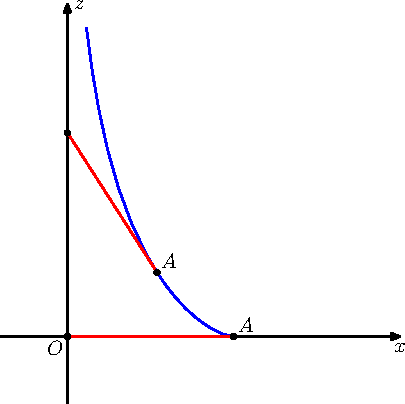
\includegraphics[scale=.8]{tractrix}\\}{}
      %\hfill\captionof{figure}{拽物线}\label{fig:tractrix}
    \end{minipage}
    \begin{solution}
      \begin{enumerate}
        \item 由图易知, 细线始终和$A$的轨迹相切. 假设$A=(x,z)$,
	  则$A$处的斜率直接计算得
          \[
            z'(x)=-\frac{\sqrt{1-x^2}}{x},\quad 0<x\leq1.
          \]
          这即表明拽物线$z=z(x)$满足常微分方程\eqref{eq:tractrix}. \score{4}

          由$z(t)=z(x(t))$, 利用复合函数求导知道
          \begin{align*}
            z'(t)&=z'(x)x'(t)=-\frac{\sqrt{1-[x(t)]^2}}{x(t)}\cdot x'(t)\\
                 &=-\sqrt{\cosh^2 t-1}\cdot \frac{-\sinh t}{\cosh^2t}
                 =\frac{\sinh^2 t}{\cosh^2t}=\tanh^2t.
          \end{align*}
          另一方面,
          \[
            z'(t)=1-\tanh't=1-\frac{1}{\cosh^2t}
            =\frac{\sinh^2 t}{\cosh^2t}=\tanh^2t.
          \]
          这表明, \eqref{eq:para-tractrix}确实满足微分方程\eqref{eq:tractrix}.
          \score{2}

          又由于$x(0)=1, z(0)=0$确实在拽物线上, 故由常微分方程的存在唯一性知
          \eqref{eq:para-tractrix}就是拽物线的参数化. \score(2)

          最后, 由拽物面是由拽物线$z=z(x)$绕着$z$轴旋转一周得到的. 
	  故其参数方程为
          \[
            \begin{cases}
              x=\sech t\cos\theta,\\
              y=\sech t\sin\theta,\\
              z=t-\tanh t,
            \end{cases}\quad
            0\leq t<+\infty,\quad 0\leq \theta\leq 2\pi
            \score{2}
          \]
        \item 我们可以将旋转面参数化为
          \[
            X(r,\theta)=\left(r\cos\theta,r\sin\theta,z(r)\right),
            0<r\leq1, 0\leq \theta\leq 2\pi,
          \]
          因此, 旋转曲面的面积微元为
          \[
            dS=\lvert X_r\times X_\theta \rvert drd\theta
            =r\sqrt{1+[z'(r)]^2}drd\theta,\score{5}
          \]
          因此, 旋转曲面的表面积为
          \[
            S=\int_0^{2\pi}d\theta\int_0^1 \lvert X_r\times X_\theta \rvert dr
            =2\pi\int_0^1r\sqrt{1+[z'(r)]^2}dr. \score{3}
          \]

          根据\eqref{eq:tractrix}, 我们得到
          \[
            \sqrt{1+z'^2(r)}=1/r,\implies S= 2\pi. \score{2}
          \]

          \textbf{法二}: 如果直接使用(a)中得到的参数方程
          \[
            X(t,\theta)
	    =\left( \sech t\cos\theta,\sech t\sin\theta,t-\tanh t \right),
            \score{2}
          \]
          则容易算出
          \[
            dS=\lvert X_t\times X_\theta \rvert dt d\theta
            =\sech t\tanh t dt d\theta
            =\frac{\sinh t}{\cosh^2t} dt d\theta.\score{5}
          \]
          因此, $\Sigma$的表面积为
          \begin{align*}
            S&=\int_0^{2\pi}d\theta\int_0^{+\infty}\sech t\tanh tdt \score{3}\\
             &=-2\pi\int_0^{+\infty} d(\sech t)
             =2\pi.\score{2}
          \end{align*}
        \item 使用\eqref{eq:para-tractrix}给出的参数化,
          \[
            X(t,\theta)=(\sech t\cos\theta,\sech t\sin\theta,t-\tanh t),\quad
            t\in[0,+\infty),\quad\theta\in[0,2\pi].
          \]
          因此,
          \[
            J=\frac{\partial(x,y)}{\partial(t,\theta)}
	    =-\sech^2 t\tanh t.\score{2}
          \]
          故体积为
          \begin{align*}
            \lvert \Omega \rvert 
            &=\iint_{x^2+y^2\leq 1}zdxdy
            =\int_0^{2\pi}d\theta\int_0^{+\infty}
            (t-\tanh t)\sech^2 t\tanh t dt,\score{5}\\
            \frac{\lvert \Omega \rvert}{2\pi}
            &=\int_0^1 (u\arctanh u-u^2) du,
            \quad(u=\tanh t, du=\sech^2 tdt)\\
            &=-\frac{1}{3}+\frac{1}{2}\int_0^1\arctanh u du^2\\
            &=-\frac{1}{3}+\frac{1}{2}
	    \left( \left. u^2\arctanh u \right\rvert_{u=0}^1
            -\int_0^1 \frac{u^2}{1-u^2}du \right),\quad 
	    (\arctanh'u=\frac{1}{1-u^2})\\
            &=-\frac{1}{3}+\frac{1}{2}
	    \left( \left. u^2\arctanh u \right\rvert_{u=0}^1
	      +1-\frac{1}{2}\int_0^1\left( \frac{1}{1-u}+\frac{1}{1+u} \right)
	    du \right)\\
            &=\frac{1}{6}+\frac{1}{2}
	    \left. \left( u^2\arctanh u
	      -\frac{1}{2}\left( -\ln(1-u)+\ln(1+u) \right) \right) 
	    \right\rvert_{u=0}^1\\
            &=\frac{1}{6}+\frac{1}{2}\lim_{u\to1^-}\left( u^2\arctanh u
            -\sqrt{\frac{1-u}{1+u}} \right).\score{3}
          \end{align*}
          将$u=\tanh t$, 代入
          \begin{align*}
            \lim_{u\to1^-}\left(u^2\arctanh u+\ln\sqrt{\frac{1-u}{1+u}}\right)
        &=\lim_{t\to+\infty}\left(t\tanh^2 t
        +\ln\sqrt{\frac{1-\tanh t}{1+\tanh t}}\right)\\
        &=\lim_{t\to+\infty}\left( t\frac{(e^{t}-e^{-t})}{e^{t}+e^{-t}}
        -\ln(\cosh t+\sinh t) \right)\\
        &=\lim_{t\to+\infty}(\frac{t(e^{t}-e^{-t})}{e^{t}+e^{-t}}-t)=0.
          \end{align*}
          因此
          \[
            \lvert \Omega \rvert=\pi/3.\score{2}
          \]
      \end{enumerate}
    \end{solution}
  \end{problem}
\end{makepart}
\end{document}
%</main>
%    \end{macrocode}
%\CheckSum{0}
%\Finale
\endinput
